\documentclass{ximera}

%\usepackage{todonotes}

\newcommand{\todo}{}

\usepackage{tkz-euclide}
\tikzset{>=stealth} %% cool arrow head
\tikzset{shorten <>/.style={ shorten >=#1, shorten <=#1 } } %% allows shorter vectors

\usepackage{tkz-tab}  %% sign charts
\usetikzlibrary{decorations.pathreplacing} 

\usetikzlibrary{backgrounds} %% for boxes around graphs
\usetikzlibrary{shapes,positioning}  %% Clouds and stars
\usetikzlibrary{matrix} %% for matrix
\usepgfplotslibrary{polar} %% for polar plots
\usetkzobj{all}
\usepackage[makeroom]{cancel} %% for strike outs
%\usepackage{mathtools} %% for pretty underbrace % Breaks Ximera
\usepackage{multicol}

\usepackage{polynom}



\usepackage[many]{tcolorbox}  %% for titled boxes
\newtcolorbox{xbox}[1]{%
    tikznode boxed title,
    enhanced,
    arc=0mm,
    interior style={white},
    attach boxed title to top center= {yshift=-\tcboxedtitleheight/2},
    fonttitle=\bfseries,
    colbacktitle=white,coltitle=black,
    boxed title style={size=normal,colframe=white,boxrule=0pt},
    title={#1}}


\usepackage{array}
\setlength{\extrarowheight}{+.1cm}   
\newdimen\digitwidth
\settowidth\digitwidth{9}
\def\divrule#1#2{
\noalign{\moveright#1\digitwidth
\vbox{\hrule width#2\digitwidth}}}





\newcommand{\RR}{\mathbb R}
\newcommand{\R}{\mathbb R}
\newcommand{\N}{\mathbb N}
\newcommand{\Z}{\mathbb Z}

%\renewcommand{\d}{\,d\!}
\renewcommand{\d}{\mathop{}\!d}
\newcommand{\dd}[2][]{\frac{\d #1}{\d #2}}
\newcommand{\pp}[2][]{\frac{\partial #1}{\partial #2}}
\renewcommand{\l}{\ell}
\newcommand{\ddx}{\frac{d}{\d x}}
\newcommand{\ddt}{\frac{d}{\d t}}

\newcommand{\zeroOverZero}{\ensuremath{\boldsymbol{\tfrac{0}{0}}}}
\newcommand{\inftyOverInfty}{\ensuremath{\boldsymbol{\tfrac{\infty}{\infty}}}}
\newcommand{\zeroOverInfty}{\ensuremath{\boldsymbol{\tfrac{0}{\infty}}}}
\newcommand{\zeroTimesInfty}{\ensuremath{\small\boldsymbol{0\cdot \infty}}}
\newcommand{\inftyMinusInfty}{\ensuremath{\small\boldsymbol{\infty - \infty}}}
\newcommand{\oneToInfty}{\ensuremath{\boldsymbol{1^\infty}}}
\newcommand{\zeroToZero}{\ensuremath{\boldsymbol{0^0}}}
\newcommand{\inftyToZero}{\ensuremath{\boldsymbol{\infty^0}}}



\newcommand{\numOverZero}{\ensuremath{\boldsymbol{\tfrac{\#}{0}}}}
\newcommand{\dfn}{\textbf}
%\newcommand{\unit}{\,\mathrm}
\newcommand{\unit}{\mathop{}\!\mathrm}
\newcommand{\eval}[1]{\bigg[ #1 \bigg]}
\newcommand{\seq}[1]{\left( #1 \right)}
\renewcommand{\epsilon}{\varepsilon}
\renewcommand{\iff}{\Leftrightarrow}

\DeclareMathOperator{\arccot}{arccot}
\DeclareMathOperator{\arcsec}{arcsec}
\DeclareMathOperator{\arccsc}{arccsc}
\DeclareMathOperator{\si}{Si}
\DeclareMathOperator{\proj}{proj}
\DeclareMathOperator{\scal}{scal}


\newcommand{\tightoverset}[2]{% for arrow vec
  \mathop{#2}\limits^{\vbox to -.5ex{\kern-0.75ex\hbox{$#1$}\vss}}}
\newcommand{\arrowvec}[1]{\tightoverset{\scriptstyle\rightharpoonup}{#1}}
\renewcommand{\vec}{\mathbf}
\newcommand{\veci}{\vec{i}}
\newcommand{\vecj}{\vec{j}}
\newcommand{\veck}{\vec{k}}
\newcommand{\vecl}{\boldsymbol{\l}}

\newcommand{\dotp}{\bullet}
\newcommand{\cross}{\boldsymbol\times}
\newcommand{\grad}{\boldsymbol\nabla}
\newcommand{\divergence}{\grad\dotp}
\newcommand{\curl}{\grad\cross}
%\DeclareMathOperator{\divergence}{divergence}
%\DeclareMathOperator{\curl}[1]{\grad\cross #1}


\colorlet{textColor}{black} 
\colorlet{background}{white}
\colorlet{penColor}{blue!50!black} % Color of a curve in a plot
\colorlet{penColor2}{red!50!black}% Color of a curve in a plot
\colorlet{penColor3}{red!50!blue} % Color of a curve in a plot
\colorlet{penColor4}{green!50!black} % Color of a curve in a plot
\colorlet{penColor5}{orange!80!black} % Color of a curve in a plot
\colorlet{fill1}{penColor!20} % Color of fill in a plot
\colorlet{fill2}{penColor2!20} % Color of fill in a plot
\colorlet{fillp}{fill1} % Color of positive area
\colorlet{filln}{penColor2!20} % Color of negative area
\colorlet{fill3}{penColor3!20} % Fill
\colorlet{fill4}{penColor4!20} % Fill
\colorlet{fill5}{penColor5!20} % Fill
\colorlet{gridColor}{gray!50} % Color of grid in a plot

\newcommand{\surfaceColor}{violet}
\newcommand{\surfaceColorTwo}{redyellow}
\newcommand{\sliceColor}{greenyellow}




\pgfmathdeclarefunction{gauss}{2}{% gives gaussian
  \pgfmathparse{1/(#2*sqrt(2*pi))*exp(-((x-#1)^2)/(2*#2^2))}%
}


%%%%%%%%%%%%%
%% Vectors
%%%%%%%%%%%%%

%% Simple horiz vectors
\renewcommand{\vector}[1]{\left\langle #1\right\rangle}


%% %% Complex Horiz Vectors with angle brackets
%% \makeatletter
%% \renewcommand{\vector}[2][ , ]{\left\langle%
%%   \def\nextitem{\def\nextitem{#1}}%
%%   \@for \el:=#2\do{\nextitem\el}\right\rangle%
%% }
%% \makeatother

%% %% Vertical Vectors
%% \def\vector#1{\begin{bmatrix}\vecListA#1,,\end{bmatrix}}
%% \def\vecListA#1,{\if,#1,\else #1\cr \expandafter \vecListA \fi}

%%%%%%%%%%%%%
%% End of vectors
%%%%%%%%%%%%%

%\newcommand{\fullwidth}{}
%\newcommand{\normalwidth}{}



%% makes a snazzy t-chart for evaluating functions
%\newenvironment{tchart}{\rowcolors{2}{}{background!90!textColor}\array}{\endarray}

%%This is to help with formatting on future title pages.
\newenvironment{sectionOutcomes}{}{} 



%% Flowchart stuff
%\tikzstyle{startstop} = [rectangle, rounded corners, minimum width=3cm, minimum height=1cm,text centered, draw=black]
%\tikzstyle{question} = [rectangle, minimum width=3cm, minimum height=1cm, text centered, draw=black]
%\tikzstyle{decision} = [trapezium, trapezium left angle=70, trapezium right angle=110, minimum width=3cm, minimum height=1cm, text centered, draw=black]
%\tikzstyle{question} = [rectangle, rounded corners, minimum width=3cm, minimum height=1cm,text centered, draw=black]
%\tikzstyle{process} = [rectangle, minimum width=3cm, minimum height=1cm, text centered, draw=black]
%\tikzstyle{decision} = [trapezium, trapezium left angle=70, trapezium right angle=110, minimum width=3cm, minimum height=1cm, text centered, draw=black]


\outcome{Understand how Riemann sums are used to find exact area.}
\outcome{Define net area.}
\outcome{Approximate net area.}
\outcome{Define the definite integral.}
\outcome{Compute definite integrals using limits of Riemann Sums.}


\title[Dig-In:]{The definite integral}

\begin{document}
\begin{abstract}
  Definite integrals arise as the limits of Riemann sums, and compute net areas.
\end{abstract}
\maketitle


In the previous sections, we've been approximating the area under a curve by treating the region as a collection of
rectangles. 

\begin{example}
	Approximate the area under the graph of $f(x)=x^2$ on the interval $[0,1]$ using right-endpoints and $n$ rectangles, for $n$ a positive integer.
	\begin{explanation}
		We'll start with the widths: $\Delta x = \frac{b-a}{n} = \frac{1}{n}$.
		
		Since we're using right-endpoints, the sample points are given by $x_k^* = a + k \Delta x = \frac{k}{n}$.
		
		The height of the $k$-th rectangle is $f(x_k^*) = \left( \frac{k}{n} \right)^2 = \frac{\answer[given]{k^2}}{n^2}$.
		
		The area of the $k$-th rectangle is $f(x_k^*)\Delta x = \left(\frac{k^2}{n^2}\right)\left( \frac{1}{n} \right) = \frac{\answer[given]{k^2}}{\answer[given]{n^3}}$.
		
		The area approximation is given by the Riemann sum.
		\begin{align*}
			\sum_{k=1}^{n} f(x_k^*) \Delta x &= \sum_{k=1}^n \frac{k^2}{n^3}\\
				&= \frac{1}{n^3} \sum_{k=1}^{n} \answer[given]{k^2} \quad \text{(We have a formula for this!)}\\
				&= \frac{1}{n^3} \left( \frac{n(n+1)(2n+1)}{6}\right)\\
				&= \frac{n(n+1)(2n+1)}{6n^3}\\
				&= \frac{(n+1)(2n+1)}{6n^2}
		\end{align*}

		The approximate area is $\frac{(n+1)(2n+1)}{6n^2}$.
	\end{explanation}
\end{example}

The benefit of doing this calculation with $n$ still variable, is that it's now easy to find the approximation for every possible value of $n$!
If we wanted to approximate the area under $f(x)=x^2$ using $4$ rectangles, we could substitute $n=4$ into this formula.
$\frac{(4+1)(2\cdot4+1)}{6(4)^2} = \frac{15}{32}$.  If we wanted to use $10$ rectangles, we can substitute $n=10$ into it.
$\frac{(10+1)(2\cdot 10+1)}{6(10)^2} = \frac{77}{200}$.

Why would we want to be able to plug in different values of $n$?  Remember how we made the approximation better and better?  By taking
more and more rectangles!  The actual area is given in the limit as $n\to \infty$.

\begin{example}
	Find the actual area under the graph of $f(x)=x^2$ on the interval $[0,1]$.
	\begin{explanation}
		We saw that the area approximation using $n$ rectangles was given by
		\[ A(n) = \frac{(n+1)(2n+1)}{6n^2} \]
		The actual area is given by
		\begin{align*}
			\lim_{n\to\infty} A(n) &= \lim_{n\to\infty} \frac{(n+1)(2n+1)}{6n^2}\\
				&= \lim_{n\to\infty} \frac{2n^2+3n+1}{6n^2} \\
				&= \lim_{n\to\infty} \frac{4n+3}{12n} \quad \text{L'Hopital's Rule}\\
				&= \lim_{n\to\infty} \frac{4}{12} \quad \text{L'Hopital's Rule}\\
				&= \answer{\frac{1}{3}}
		\end{align*}
	\end{explanation}
\end{example}

All of the functions we have been examining have been positive.  What changes if $f$ is negative in the region?

Let's look at $f(x) = \cos(x)$ on $[0, \pi]$ with $n=4$ using midpoints.
$\Delta x = \frac{\pi}{4}$, so the regular partition is $\left[ 0 \, , \, \frac{\pi}{4} \right]$, $\left[ \frac{\pi}{4} \, , \, \frac{\pi}{2} \right]$, $\left[ \frac{\pi}{2} \, , \, \frac{3\pi}{4} \right]$, and 
$\left[ \frac{3\pi}{4} \, , \, \pi \right]$, giving us midpoints $x_1^* = \frac{\pi}{8}$, $x_2^* = \frac{3\pi}{8}$, $x_3^* = \frac{3\pi}{8}$, and $x_4^*=\frac{7\pi}{8}$.
%pi/4 \approx 0.7854
\begin{image}
  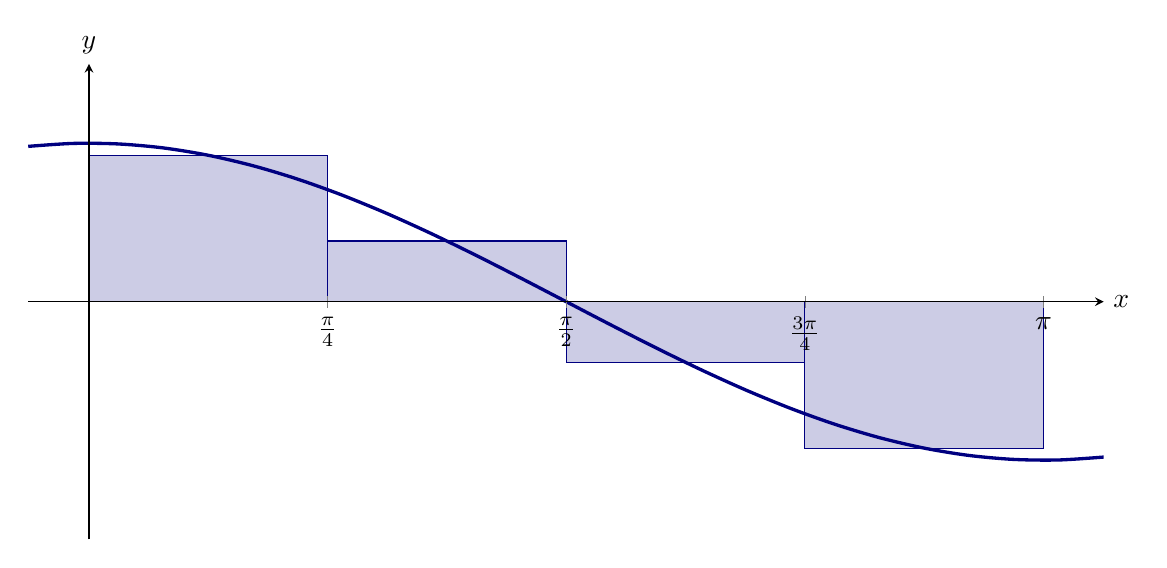
\begin{tikzpicture}[
      declare function = {f(\x) = cos(deg(\x));}]
    \begin{axis}[  
        domain=-.2:3.34, xmin =-.2,xmax=3.34,ymax=1.5,ymin=-1.5,
        width=6in, height=3in,
        xtick={0,0.7854,1.5708,2.3562, 3.1416},
        xticklabels={0, $\frac{\pi}{4}$, $\frac{\pi}{2}$, $\frac{3\pi}{4}$, $\pi$},
        ytick style={draw=none},
        yticklabels={},
        axis lines=center, xlabel=$x$, ylabel=$y$,
        every axis y label/.style={at=(current axis.above origin),anchor=south},
        every axis x label/.style={at=(current axis.right of origin),anchor=west},
        axis on top,
      ]
      \foreach \rectnumber in {1,2,3,4}
               {
                 \addplot [draw=penColor,fill=fillp] plot coordinates
                          {({(\rectnumber - 1) * 0.7854},{f(0.3927+(\rectnumber - 1) * 0.7854)})
                            ({(\rectnumber) * 0.7854},{f(0.3927+(\rectnumber - 1) * 0.7854) })} \closedcycle;
               };
               \addplot [very thick,penColor, smooth] {f(x)};
               \node[fillp!50!black] at (axis cs:3.5,1) {\huge$\mathsf{1}$};
    \end{axis}
  \end{tikzpicture}
\end{image}

In the Riemann sum
\[ f(x_1^*)\Delta x + f(x_2^*)\Delta x + f(x_3^*)\Delta x + f(x_4^*)\Delta x, \]
the first two terms $f(x_1^*)\Delta x$ and $f(x_2^*)\Delta x$ are the areas of the first two rectangles.
Notice that $f(x_3^*)$ and $f(x_4^*)$ are negative!  They are not the heights of their rectangles.  They
are the opposite of the heights.  That means $f(x_3^*)\Delta x$ and $f(x_4^*)\Delta x$ are not the areas of those rectangles.  
They are the opposite of those areas.  The Riemann sum is adding the areas of the first two rectangles, then subtracting the
areas of the last two rectangles.

This same situation occurs whenever our function is negative.  The areas of the corresponding rectangles are being subtracted, not added.

\begin{definition}\index{net area}
	The \dfn{net area} of a region is the area above the $x$-axis minus the area below the $x$-axis.
\end{definition}
The Riemann sum is not calculating the approximate area, but the net area.


\begin{example}
	Compute the net area bounded by the graph of $f(x) = \cos(x)$ and the $x$-axis between $x=0$ and $x=\pi$.
	\begin{explanation}
		Let's look at the graph.
		\begin{image}
 	 	\begin{tikzpicture}[declare function = {f(\x) = cos(deg(\x));}]
    			\begin{axis}[  
        				domain=-.2:3.34, xmin =-.2,xmax=3.34,ymax=1.5,ymin=-1.5,
        				width=6in, height=3in,
        xtick={0,0.7854,1.5708,2.3562, 3.1416},
        xticklabels={0, $\frac{\pi}{4}$, $\frac{\pi}{2}$, $\frac{3\pi}{4}$, $\pi$},
        ytick style={draw=none},
        yticklabels={},
        axis lines=center, xlabel=$x$, ylabel=$y$,
        every axis y label/.style={at=(current axis.above origin),anchor=south},
        every axis x label/.style={at=(current axis.right of origin),anchor=west},
        axis on top,
      ]
          \addplot [very thick,penColor, smooth] {f(x)};
           \node[fillp!50!black] at (axis cs:3.5,1) {\huge$\mathsf{1}$};
    \end{axis}
  \end{tikzpicture}
\end{image}
	The area above the $x$-axis and the area below the $x$-axis are exactly the same.  That means the
	net area is $\answer[given]{0}$.
	\end{explanation}
\end{example}



Remember that when we setup our Riemann sum to approximate the areas, we had a choice on what sample points to use.
We could use left-endpoints, right-endpoints, midpoints, a combination of the three, or any other possible points we wished.
Different choices of sample points leads to different values for the Riemann sums.

\begin{definition}\index{integral}\index{integrable}\index{definite integral}
	A function $f$, defined on an interval $[a,b]$, is called \dfn{integrable} on $[a,b]$ if
	$\displaystyle \lim_{n\to\infty} \sum_{k=1}^n f(x_k^*) \Delta x$ exists and has the same
	value for ALL choices of sample points, $x_k^*$.  If $f$ is integrable on $[a,b]$, this
	limit is called the \dfn{definite integral of $f$ from $x=a$ to $x=b$}, and denoted by
	\[ \int_a^b f(x) \d x \]
\end{definition}

To say it another way, if we have an integrable function, the difference between those sample points disappears once
we take the limit, and this limit is the actual net area of the region.

Whenever we are working with an integrable function, the definite integral $\int_a^b f(x) \d x$ makes sense, but which functions are integrable?  The next theorem tells us that most of
the functions we deal with are.
\begin{theorem}
If $f$ is continuous on $[a,b]$, then $f$ is integrable on $[a,b]$.  If $f$ is bounded on $[a,b]$ with only finitely many discontinuities, then $f$ is integrable on $[a,b]$.
\end{theorem}


\begin{question}
Consider the following graph of $y=f(x)$:
\begin{image}
  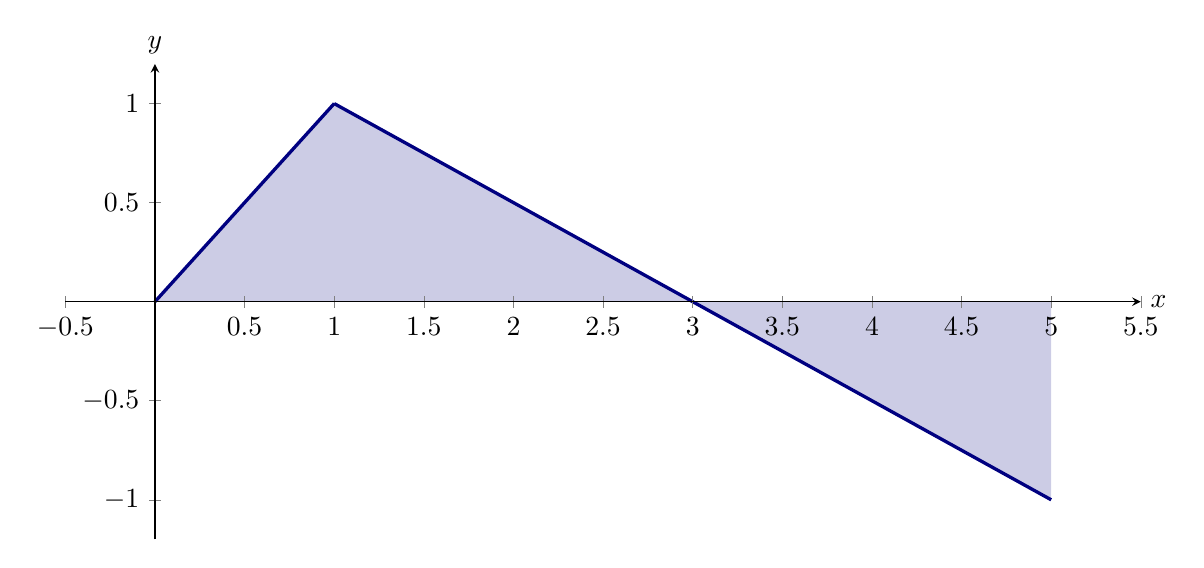
\begin{tikzpicture}
    \begin{axis}[
        width=6in,
        height=3in,
        xmin=-.5, xmax=5.5,ymin=-1.2,ymax=1.2,domain=0:6,
        axis lines =center, xlabel=$x$, ylabel=$y$,
        every axis y label/.style={at=(current axis.above origin),anchor=south},
        every axis x label/.style={at=(current axis.right of origin),anchor=west},
        axis on top,
    ] 
      \addplot [draw=none, %pattern=north west lines, pattern color=blue,
        fill=fillp,
        domain=0:1] {x} \closedcycle;
      \addplot [draw=none, %pattern=north west lines, pattern color=blue,
        fill=fillp,
        domain=1:5] {1.5-x/2} \closedcycle;
      
      \addplot [penColor,very thick,domain=0:1] {x};
      \addplot [penColor,very thick,domain=1:5] {1.5-x/2};
  \end{axis}
  \end{tikzpicture}
\end{image}
Compute:
\begin{enumerate}
	\item $\int_0^3 f(x) \d x \begin{prompt}= \answer{1.5}\end{prompt}$
	\item $\int_3^5 f(x) \d x \begin{prompt}= \answer{-1}\end{prompt}$
	\item $\int_0^5 f(x) \d x \begin{prompt}= \answer{0.5}\end{prompt}$
\end{enumerate}
\begin{hint}
	  Use the formula for the area of a triangle.
\end{hint}
\begin{hint}
 	Remember, we are dealing with ``signed'' area here:
  \begin{image}
  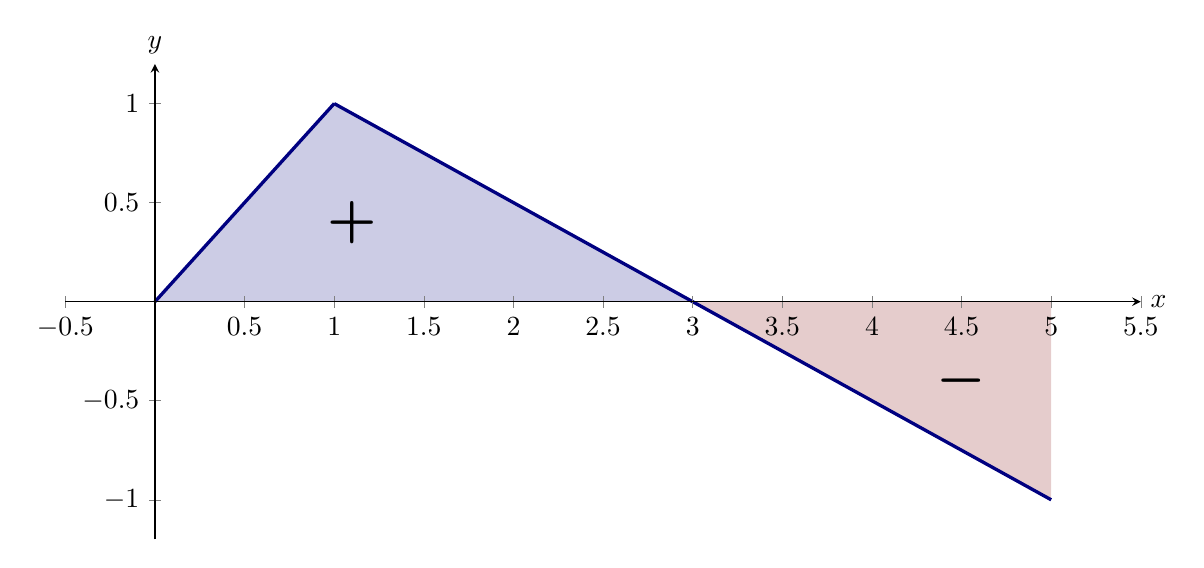
\begin{tikzpicture}
    \begin{axis}[
        width=6in,
        height=3in,
        xmin=-.5, xmax=5.5,ymin=-1.2,ymax=1.2,domain=0:6,
        axis lines =center, xlabel=$x$, ylabel=$y$,
        every axis y label/.style={at=(current axis.above origin),anchor=south},
        every axis x label/.style={at=(current axis.right of origin),anchor=west},
        axis on top,
    ] 
      \addplot [draw=none, fill=fillp,domain=0:1] {x} \closedcycle;
      \addplot [draw=none, fill=fillp,domain=1:3] {1.5-x/2} \closedcycle;
      \addplot [draw=none, fill=filln,domain=3:5] {1.5-x/2} \closedcycle;
      
      \addplot [penColor,very thick,domain=0:1] {x};
      \addplot [penColor,very thick,domain=1:5] {1.5-x/2};
      \node at (axis cs:1.1,.4) [textColor] {\scalebox{2}{$\boldsymbol+$}};
      \node at (axis cs:4.5,-.4) [textColor] {\scalebox{2}{$\boldsymbol-$}};
  \end{axis}
  \end{tikzpicture}
\end{image}
\end{hint}
\end{question}



\begin{example}
	Evaluate: $\displaystyle \int_0^2 (x^3-2x) \d x$.
	\begin{explanation}
		$f(x)=x^3-2x$ is continuous everywhere, so it is integrable on $[0,2]$.  That means this definite integral is given by the limit of Riemann sums.
		
		We start by computing the right Riemann sum using $n$ rectangles. 
		
		\begin{align*}
			\Delta x &= \answer[given]{\frac{2}{n}} \\ \\
			x_k^* &= \answer[given]{\frac{2k}{n}}\\ \\
			f(x_k^*) &= \left( \frac{2k}{n}\right)^3 - 2\left(\frac{2k}{n}\right)\\
				&= \frac{8}{n^3}k^3 - \frac{4}{n}k \\  \\
			f(x_k^*)\Delta x &= \left(\frac{8}{n^3}k^3 - \frac{4}{n}k\right) \left( \frac{2}{n}\right)\\
				&= \frac{16}{n^4}k^3 - \frac{8}{n^2}k
		\end{align*}				
		\begin{hint}
			\begin{align*}
				\Delta x &= \frac{b-a}{n}\\
				x_k^* &= a + k\Delta x
			\end{align*}
		\end{hint}
		The Riemann sum is given by:
		\begin{align*}
			\sum_{k=1}^n f(x_k^*)\Delta x &= \sum_{k=1}^n \left(\frac{16}{n^4}k^3 - \frac{8}{n^2}k \right)\\
				&= \sum_{k=1}^n \frac{16}{n^4}k^3 - \sum_{k=1}^n \frac{8}{n^2}k \\
				&= \frac{16}{n^4} \sum_{k=1}^n \answer[given]{k^3} - \frac{8}{n^2}\sum_{k=1}^n \answer[given]{k} \\
				&= \frac{16}{n^4} \left( \frac{n^2(n+1)^2}{4} \right) - \frac{8}{n^2}\left( \frac{n(n+1)}{2} \right) \\
				&= \frac{16n^2(n+1)^2}{4n^4} - \frac{8n(n+1)}{2n^2} \\
				&= \frac{4(n+1)^2}{n^2} - \frac{4(n+1)}{n}
		\end{align*}
		The definite integral is the limit of these.
		\begin{align*}
			\int_0^2 (x^3-2x) \d x &= \lim_{n\to \infty}\sum_{k=1}^n f(x_k^*)\Delta x \\
				&= \lim_{n\to\infty} \left(\frac{4(n+1)^2}{n^2} - \frac{4(n+1)}{n}\right) \\
				&= \lim_{n\to\infty} \frac{4(n+1)^2}{n^2} - \lim_{n\to\infty} \frac{4(n+1)}{n} \\
				&= \answer[given]{4} - \answer[given]{4}\\
				&= \answer[given]{0}
		\end{align*}
	\end{explanation}
\end{example}








\end{document}
